\documentclass[10pt, letterpaper, twocolumn]{article}
\usepackage[english]{babel}

\usepackage[pagenumbers]{cvpr}
\usepackage[pagebackref,breaklinks,colorlinks]{hyperref}

\usepackage{amsmath}
\usepackage{amssymb}

\usepackage{graphicx}
\usepackage{multirow}

\usepackage{lipsum}

\usepackage{stfloats}

\usepackage[none]{hyphenat}

\begin{document}

\title{Hyperbolic Vision Transformers}
\author{Yuriy Sosnin\\HSE University}
\maketitle

\begin{abstract}
This paper evaluates the hyperbolic embeddings methodology proposed by Ermolov et al. \cite{ermolov_hyperbolic_2022} within a metric learning framework, employing the vanilla Triplet loss. While we do not achieve state-of-the-art results, we demonstrate that Hyperbolic embeddings can outperform standard Euclidean embeddings in some scenarios even with minimal adjustments to default metric learning pipeline. Additionally, we propose a fully Hyperbolic Vision Transformer operating on the hyperbolic patch space. We do not obtain training results, leaving it as future work for exploration.
\end{abstract}

\newcommand{\dotproduct}[1]{\langle #1 \rangle}
\newcommand{\norm}[1]{\lVert #1 \rVert}
\newcommand{\sbrakets}[1]{\left( #1 \right)}

\section{Introduction}

Representation learning, also known as feature learning, aims to automatically discover meaningful and informative representations of raw data. Traditional machine learning approaches often require manually engineered features, which can be time-consuming and domain-specific. Representation learning, on the other hand, leverages the power of deep neural networks to extract high-level features from raw data, enabling the model to learn directly from the raw input. By learning representations that capture the underlying structure and patterns in the data, representation learning has shown great success in various tasks such as image recognition, natural language processing, and recommendation systems.

Inductive biases about the data and the space in which object representations are hypothesized to lie can greatly enhance model efficiency and yield superior results. One natural property observed in many real-world datasets is the presence of hierarchy. For instance, social networks exhibit power law distribution, small diameter, and high clustering -- properties naturally emerging from hyperbolic geometry \cite{clauset_hierarchical_2008, krioukov_hyperbolic_2010}. Natural Language domain consists of data that have tree-like structures -- words form dependency trees inside sentences, and hierarchical semantic trees in the whole language \cite{tifrea_Poincare_2018}. ImageNet is in essence hierarchical \cite{deng_imagenet_2009}.

Most Neural Representation models are by default Euclidean, and Euclidean spaces are inherently limited in capturing hierarchy. It is proven that Euclidean space can not isometrically embed a tree, even with a bounded number of dimensions. In contrast, \emph{Hyperbolic} spaces have properties that allow them to embed trees naturally. Hyperbolic space has negative curvature, it expands exponentially with distance from the origin, and therefore are able to embed trees with low distortion \cite{sarkar_low_2012}. These characteristics make Hyperbolic spaces an appealing inductive bias to incorporate into representation models.

The field of Hyperbolic Neural Networks has been rapidly developed in recent years. Mostly it has been focused on NLP, but it has been demonstrated that Computer Vision applications can also benefit from these advancements \cite{khrulkov_hyperbolic_2020}. In our work, we follow the approach of \cite{ermolov_hyperbolic_2022}. They propose to use pre-trained Vision Transformers (ViT) \cite{dosovitskiy_image_2021} as Euclidean feature extractors, and project the resulting representations into Poincar\'e Ball model of hyperbolic space. We evaluate ViT in hyperbolic space on a default pipeline with Triplet loss, and propose (without experiments) fully hyperbolic architecture. Additionally, we discuss the limitations associated with our implementation.

The rest of the paper is organized as follows. In section \ref{sec:hnn} we briefly introduce Poincar\'e Ball model of hyperbolic space, and how are necessary neural network operations defined in it. Section \ref{sec:method} describes our empirical procedure, introduces ViT and briefly discusses Metric Learning. We then present our results. In section \ref{sec:fully} we propose a fully hyperbolic Vision Transformer and explain why we failed to achieve results with it. Sections \ref{sec:ref} and \ref{sec:concl} briefly mention related literature and conclude, respectively.

\section{Neural Networks in Hyperbolic Space}\label{sec:hnn}

\subsection{Hyperbolic Space}

Hyperbolic space is a smooth Riemannian manifold with constant negative sectional curvature. As Hyperbolic space can not be naturally embedded into Euclidean space, several isometric models are used to represent it, among which the most popular in ML applications is Poincar\'e Ball. Formally, Poincar\'e Ball is a pair of n-dimensional open ball $\mathbb{B}^n_c = \{\mathbf{x} \in \mathbb{R}^n: c \norm{\mathbf{x}} < 1 \}$ where $c$ is space curvature, and a Riemannian metric tensor $g^{\mathbb{D}} = \lambda_c^2 g^E$ with conformal factor $ \lambda_c = \frac{2}{1-c \norm{x}^2}$.

A framework of gyrovector spaces allows us to define hyperbolic M\"obius addition and scalar multiplication \cite{ungar_analytic_2008,ungar_gyrovector_2009}, given by

\begin{equation}\label{eq:add}
    \mathbf{u} \oplus_c \mathbf{v} = \frac{ (1 + 2c \dotproduct{\mathbf{u}, \mathbf{v}} + c \norm{\mathbf{v}}^2) \mathbf{u} + (1 - c \norm{\mathbf{u}}^2) \mathbf{v}} {1 + 2c \dotproduct{\mathbf{u}, \mathbf{v}} + c^2 \norm{\mathbf{u}}^2 \norm{\mathbf{v}}^2 }
\end{equation}

Distance between two points in hyperbolic space is therefore defined as follows:

\begin{equation}\label{eq:dist}
    D_{hyp}(\mathbf{x}, \mathbf{y}) = \frac{2}{\sqrt{c}} \mathrm{arctanh}(\sqrt{c} \norm{-\mathbf{x} \oplus_c \mathbf{y}})
\end{equation}

A Riemannian manifold is locally represented by an n-dimensional Euclidean space called Tangent space. Logarithmic map defines a mapping $\log_\mathbf{x}^c: \mathcal{M} \rightarrow T_\mathbf{x}{\mathcal{M}}$ from the manifold to its tangent space at point $x$. Respectively, Exponential map at point $\mathbf{x}$ defines and inverse mapping from Tangent space to the manifold:

\begin{equation}\label{eq:exp}
    \exp_\mathbf{x}^c(\mathbf{v}) = \mathbf{x} \oplus_c \bigg(\tanh \bigg(\sqrt{c} \frac{\lambda_\mathbf{x}^c \norm{\mathbf{v}}}{2} \bigg) \frac{\mathbf{v}}{\sqrt{c}\norm{\mathbf{v}}}\bigg)
\end{equation}

In most applications, $\mathbf{x}$ is usually set to $\mathbf{0}$, the origin of the space, simplifying the computation.

\subsection{Hyperbolic Neural Networks}

Exploration of hyperbolic spaces in deep learning started from the work of Ganea et al., where they first formulated most neural network operations on Poincar\'e ball \cite{ganea_hyperbolic_2018}.

Matrix-vector multiplication for linear layer is performed in tangent space with Euclidean parameters: first, hyperbolic vector is logarithmically mapped to tangent space; there, matrix multiplication is performed; the result is mapped back on the manifold with exponential map and bias is added using gyrovector addition \cite{ganea_hyperbolic_2018}.

\begin{equation}
    h^c(x) = \exp_\mathbf{0}^c(\mathbf{W}(\log_\mathbf{0}^c(x))) \oplus_c \mathbf{b}
\end{equation}

Activation functions are calculated in tangent space as well:

\begin{equation}\label{eq:mobius_version}
    f^c(x) = \exp_\mathbf{0}^c(f(\log_\mathbf{0}^c(x)))
\end{equation}

Some authors hypothesized if activation functions are even needed in hyperbolic setting as matrix multiplications are already non-linear, and there is no need to avoid collapsing several "linear" layers into one.

Those formulations are sufficient for default fully-connected networks, however, to define Transformers in hyperbolic space we need more, namely, aggregation operation for self-attention and concatenation-split for making multi-head self-attention.

Self-attention layer consists of two essential parts: \emph{relation} stage, i.e. calculation of attention weights between queries and keys, and \emph{aggregation} of values with attention weights \cite{vaswani_attention_2017}. In standard Transformer architecture attention weight is SoftMax over scalar products between queries and keys; in hyperbolic case, natural metric of similarity is hyperbolic distance (\ref{eq:dist}) \cite{gulcehre_hyperbolic_2018}. Therefore, relation between query $q$ and key $k$ is calculated as follows:

\begin{equation}
    f^c(\mathbf{q}, \mathbf{k}) = -D^c(\mathbf{q}, \mathbf{k}) - \beta
\end{equation}

where $D$ is hyperbolic distance from equation \ref{eq:dist} and $\beta$ is a parameter.

Defining aggregation (weighted addition) is more difficult as it does not have a natural close form in Poincar\'e ball. Some papers use Fr\'echet mean \cite{lou_differentiating_2021} or even perform calculation in tangent space \cite{micic_hyperbolic_2018}.
However, as Klein model has a close-form, it is possible to redefine the operation for Poincar\'e ball as proposed in \cite{shimizu_hyperbolic_2021}.

\begin{equation}
    h^c(\mathbf{v}, \mathbf{\alpha}) = \frac{1}{2}\otimes_{c}\sbrakets{\frac{(\sum^N_{i=1}\alpha_i)\lambda^{c}_{\mathbf{v}_i}\mathbf{v}_i}{\sum^N_{i=1}\left|\alpha_i\right|\sbrakets{\lambda^{c}_{\mathbf{v}_i} - 1}}}
\end{equation}

where $\mathbf{v_i}$ are value vectors to be aggregated, $\alpha_i$ are scalar weights.

Split and concatenation are defined accordingly in \cite{shimizu_hyperbolic_2021}. With these operations we can extend self-attention to multiple heads.

\subsection{Optimization}

Having parameters in non-Euclidean spaces requires special optimization techniques. Gradient Descent update on Riemannian manifolds is defined the following way ($H$ is Riemannian gradient of the loss) \cite{bonnabel_stochastic_2013, becigneul_riemannian_2019}:

\begin{equation}
    w_{t+1}=\exp_{w_t}(-{\gamma_t} H(z_t,w_t))
\end{equation}

It has been noticed that Gradient Descent on parameters in Hyperbolic space exhibits numerical instability and often requires extra 64-bit precision \cite{mishne_numerical_2023}. A parallel idea is using feature clipping each time a Euclidean vector is exponentially mapped into Poincar\'e Ball, i.e. restrict the norm to some max radius $r$ \cite{guo_clipped_2022}.

\section{Method}\label{sec:method}

\begin{figure*}
    \begin{center}
    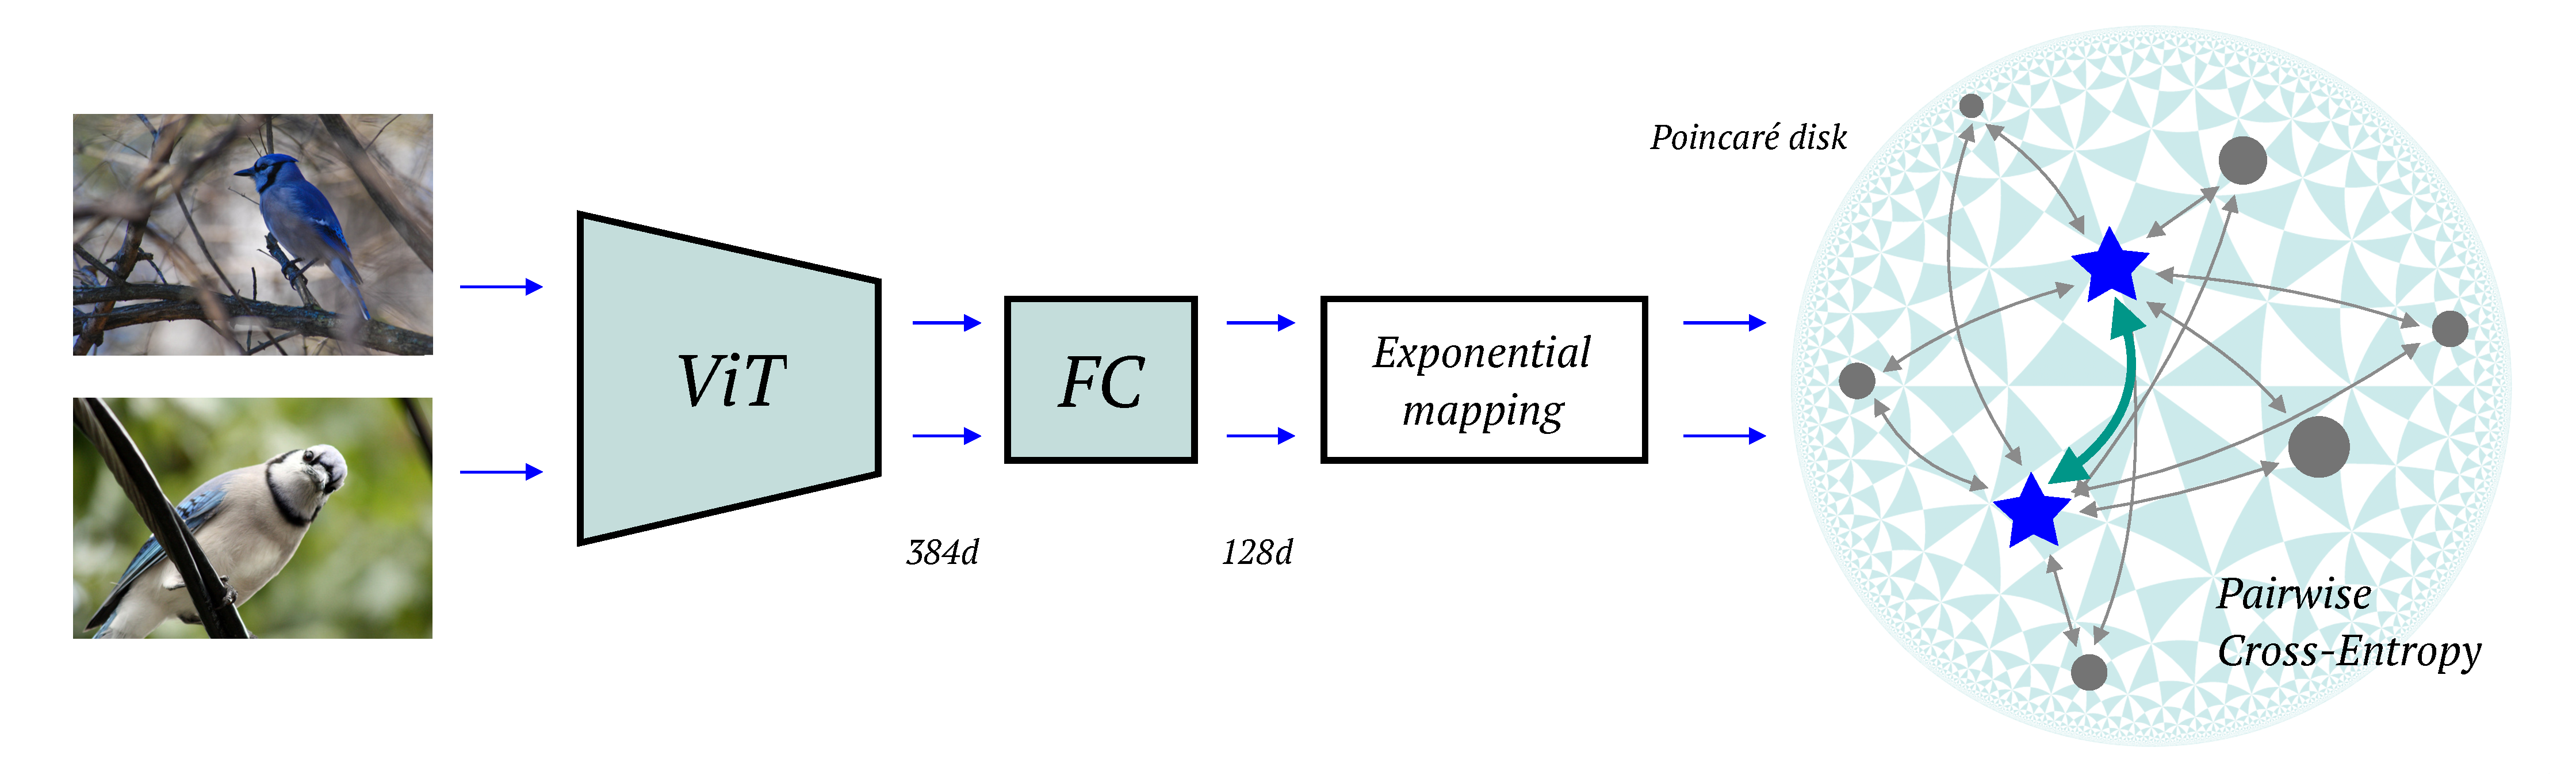
\includegraphics[width=\linewidth]{scheme.pdf}
    \caption{A pipeline for CV metric learning proposed by \cite{ermolov_hyperbolic_2022}. First, ViT extractor produces embeddings for images, then they are mapped to hyperbolic space, and distance loss calculation is performed there.}
    \label{fig:scheme}
    \end{center}
\end{figure*}

We evaluate hyperbolic embeddings methodology from \cite{ermolov_hyperbolic_2022} in metric learning framework with vanilla Triplet loss, instead of their proposed cross-entropy-like loss.
The idea is to extract representations from images using a normal Euclidean model, then map those representations into a hyperbolic space, and evaluate similarity for metric learning there. This approach offers several advantages: first, all model parameters are Euclidean, eliminating the need for Riemannian optimization and mitigating associated challenges; second, pre-trained model weights can be utilized. Still, in section \ref{sec:fully} we propose a fully hyperbolic approach, where the model itself operates on points in hyperbolic space.

\subsection{Vision Transformer}

In this section, we introduce model architecture that we employ for our experiments. Vision Transformer (ViT) \cite{dosovitskiy_image_2021, vaswani_attention_2017} is an attention-base architecture extends the successful Transformer Encoder to the domain of Computer Vision. To represent image as tokens, it is split into small non-overlapping patches (16x16 or 32x32 are popular choices), and each patch is linearly projected into a n-dimensional model space. The resulting vectors are augmented with positional encoding and fed into standard BERT-like Transformer Encoder architecture \cite{devlin_bert_2019}. To achieve the whole image representations, special [CLS] token is prepended at the bottom of the model, and its representation from the last layer is as image representation.

ViTs come in different varieties, depending on representation dimension size, number of layers and heads (base, small, large), as well as pretraining procedures.
Default ViT is pretrained on classification task on ImageNet \cite{deng_imagenet_2009}. Another prominent approach, DINO, is am unsupervised contrasive learning framework that trains a model to correctly distinguish two augmented versions of one image from random other images \cite{caron_emerging_2021, oquab_dinov2_2023}. We reference them later as ViT and DINO respectively.

\subsection{Metric Learning}

Metric Learning is a Deep Learning approach which focuses on learning a geometrically convenient embedding space for a given domain. Unlike of classification task, striving to infer a hyperplane which would separate classes in model representation space, metric learning directly optimizes this space so that similar instances are located closer to each other than dissimilar ones, according to some distance metric. It allows to easily expand models to new unseen classes, as well as solving general learning-to-rank problems. Inference is usually performed with a simple kNN in the embedding space.

Usual similarity metric is either standard Euclidean distance or so-called cosine similarity, a dot-product of normalized embedding vectors (which is equivalent to cosine of distance on a sphere). Following \cite{ermolov_hyperbolic_2022}, we instead use hyperbolic distance (\ref{eq:dist}) as similarity metric between embeddings, preliminarily exponentially mapped into hyperbolic space. It is hypothesized that many real-life datasets, and especially image datasets, are hierarchical in nature, and that employing a more appropriate manifold as inductive bias would make models more efficient and yield better results \cite{khrulkov_hyperbolic_2020}.

While \cite{ermolov_hyperbolic_2022} use a novel cross-entropy based loss, we strive to evaluate the hyperbolic space together with a classic Triplet loss pipeline \cite{hermans_defense_2017}.
The triplet loss is designed to minimize the distance between an anchor point and a positive sample, while maximizing the distance between the anchor point and a negative sample. It considers a tuple of samples $(a,p,n)$, where $a$ is the anchor instance, $p$ is the positive instance associated with the same class as the anchor, and $n$ is the negative instance from a different class. The triplet loss is formulated as:

\begin{equation}
L(a, p, n) = ReLU(\alpha + D(a, p) - D(a, n))
\end{equation}

where $D(a, p)$ and $D(a, n)$ are the similarities between anchor-positive and anchor-negative pairs (in our case, hyperbolic distances), and $\alpha$ is the margin. The margin enforces that negative samples should be at least farther away from positive samples by $\alpha$ distance. In standard "all triplets" scenario, all combinations of $a, p, n$ are mined from batch and processed at each iteration.

\section{Empirical Results}

\subsection{Data}

We evaluate the performance of our models on two popular metric learning benchmark datasets.

\textbf{CUB-200-2011:} The CUB dataset \cite{wah_caltech-ucsd_2011} consists of 11,788 images from 200 bird species. Each class contains approximately 30 to 60 images per species. Following the standard procedure, we split the dataset in half by classes, setting classes 1-100 as training set and 101-200 as validation set.

\textbf{Stanford Cars:} The Stanford Cars dataset \cite{krause_3d_2013} comprises 16,185 images from 196 car classes, with each class containing about 50 to 80 images. Similarly, we set first 96 classes as training subset and keep the rest for validation.

\subsection{implementation Details}

% Please add the following required packages to your document preamble:
% \usepackage{multirow}
\begin{table*}[t!]
    \centering
    \begin{tabular}{l|l|llll|llll}
    \multirow{2}{*}{Model} & \multirow{2}{*}{Dim} & \multicolumn{4}{l|}{CUB-200-2011}  & \multicolumn{4}{l}{Stanford Cars} \\
                           &                      & 1    & 2    & 4    & 8    & 1      & 2      & 4      & 8      \\ \hline
    DINO-Hyperbolic        & 128                  & 74.6 & 84.0 & 90.2 & 94.5 & 78.1   & 87.8   & 93.0   & 96.6   \\
    DINO-Sphere            & 128                  & 77.9 & 86.7 & 91.7 & 95.1 & 79.5   & 87.4   & 92.2   & 95.6   \\
    DINO-Hyperbolic        & 384                  & 78.0 & 86.2 & 92.1 & 95.6 & 79.6   & 88.0   & 93.2   & 94.3   \\
    DINO-Sphere            & 384                  & 77.6 & 86.6 & 91.7 & 95.1 & 79.6   & 87.6   & 93.4   & 96.2   \\ \hline
    ViT-Hyperbolic         & 128                  & 58.6   & 70.1   & 81.1   & 89.0   & 64.1   & 74.9   & 84.7   & 92.1   \\
    ViT-Sphere             & 128                  & 67.2   & 79.0   & 86.4   & 91.5   & 63.4   & 75.6   & 85.0   & 91.5   \\
    ViT-Hyperbolic         & 384                  & 60.3   & 71.8   & 82.9   & 89.7   & 65.4   & 76.2   & 85.8   & 92.5   \\
    ViT-Sphere             & 384                  & 67.9   & 79.0   & 87.2   & 93.0   & 65.7   & 75.9   & 85.2   & 92.3
    \end{tabular}
    \caption{Experimental results. Columns represent $k$ values 1, 2, 4, 8 for Recall@$k$.}
    \label{tab:results}
\end{table*}

We utilize ViT-Small as an encoder and compare two types of pretraining: standard classification (ViT) and contrasive learning (DINO). Unlike \cite{ermolov_hyperbolic_2022}, we do not freeze patch embeddings. The resulting 384-dimensional representation is projected into 128, 256 and 384-dimensional space, and then mapped either onto a sphere (by normalizing them) or into hyperbolic space. In hyperbolic space, we use hyperbolic distance as discussed earlier; on a sphere, we use cosine similarity (\ref{eq:dot}).

\begin{equation}\label{eq:dot}
    D_{sph}(\mathbf{x},\mathbf{y}) = - \dotproduct{\mathbf{x}, \mathbf{y}}
\end{equation}

We use a curvature parameter $c = 0.1$, and clipping radius $r = 2.3$.

To evaluate the performance of metric learning algorithms, we report Recall@$k$. Recall@$k$ represents the proportion of instances in the top $k$ retrieved neighbors that are of the same class as the query instance. The neighbors are selected according to appripriate distance $D$ -- $D_{hyp}$ in case of hyperbolic projection and $D_{sph}$ in case of sphere.

We use the AdamW optimizer \cite{loshchilov_decoupled_2019} with a learning rate of $1e-5$ for DINO and $3e-5$ for ViT-Small, with the weight decay value of $0.01$. We sample 8 labels and 20 instances for each label and form every batch this way. We run training for 30 epochs on both datasets. Data augmentations include random crop resizing of the image to 224x224 using bicubic interpolation with a random horizontal flip; test images are resized to 224 on the smaller side and centered cropped to 224x224. As we are not dealing with any non-Euclidean parameters, we use default 32-bit precision.

We perform our experiments in PyTorch \cite{paszke_pytorch_2019}, using Open Metric Learning framework \cite{noauthor_oml-teamopen-metric-learning_2023} for metric learning parts of our code, and geoopt \cite{kochurov_geoopt_2020} as geometric optimization implementation.

\subsection{Results}

Table \ref{tab:results} presents experimental results for our approach. Rows represent different model variations and columns encode values for Recall@$k$.

We did not manage to achieve competitive results comparable to those reported in \cite{ermolov_hyperbolic_2022}. Most likely, vanilla triplet loss, comparing at each instance only three objects, lacks the expressiveness of N-pair cross entropy loss, comparing each object with all objects of different classes from the batch at once. Moreover, our vanilla ViT results substantially underperform results obtained with the DINO backbone. We can hypothesize that contrasive pretraining yields a more favorable embedding space in context of distance-based triplet loss, and this difference is less pronounces in method of \cite{ermolov_hyperbolic_2022}.

Despite this, we can still compare Spherical representation and Hyperbolic representations. As we can see, it is not clear from our results that hyperbolic space is substantially better across all cases. Hyperbolic representations achieve better results in case of CUB dataset in higher embedding dimension.

\section{Fully-Hyperbolic Vision Transformer}\label{sec:fully}

% \begin{figure*}[ht!]
%     \includegraphics[width=\textwidth]{image.png}
%     \caption{Left: hierarchical structure in image space. Right: hierarchical structure in \emph{patch} space.}
% \end{figure*}

The idea of mapping image representations into hyperbolic space is that those representations exhibit hierarchical structure \cite{khrulkov_hyperbolic_2020}. However, we can hypothesize that the space of \emph{patches} that Vision Transformer operates on, which are of course images as well, is even more hyperbolic. Say, a background depicting grass is not really discriminative of the image class, and should intuitively reside near the origin of the space. Furthermore, some features can be associated with several distinct classes, and should be located further. Finally, specific features that allow to distinguish a specific class are the outermost branches in this hierarchy.

Indeed, one of the first applications of hyperbolic Machine Learning was embedding \emph{words}, which later prompted fully hyperbolic NLP Transformers \cite{ganea_hyperbolic_2018, nickel_learning_2018}.

We hypothesize that including this inductive bias into a Vision Transformer architecture itself can improve the parameter efficiency and therefore achieve even better results. In other words, instead of mapping the whole image representation, we can map \emph{patch} representations at the very beginning of the model.

As we discussed in section \ref{sec:hnn}, we have all the necessary parts to implement fully hyperbolic Transformers, operating with inputs that lie in hyperbolic space. The only part lacking is Layer Normalization \cite{ba_layer_2016}, but we decide to implement our model without it.

As discussed earlier, fully-hyperbolic models are subject to computational instability and essentially require 64-bit precision to train. We try to train our model with 64-bit precision, but Tesla V100 GPU with 80 GB RAM goes out of memory. In an attempt to fix these huge memory requirements, we derive gradients for some hyperbolic operations explicitly.
However, that yields even worse results -- it turns out PyTorch default autograd is more efficient.

We reduce precision to 32 bit and manage to run a training procedure from section \ref{sec:method}. However, another important difference from those experiments that we can not use pre-trained weights anymore. Indeed, it turns out that initializing the model with pre-trained weights yields no better results than initializing with random weights. This highlights the need to employ an extensive pretraining akin to \cite{dosovitskiy_image_2021,caron_emerging_2021,oquab_dinov2_2023}. We decide to leave this to future work.

\section{Related Literature}\label{sec:ref}

Recently hyperbolic Neural Networks have become a prominent stream of literature. Despite early applications focused on NLP tasks \cite{ganea_hyperbolic_2018}, Computer Vision have caught up as well. As mentioned earlier, image datasets tend to exhibit a high degree of hyperbolicity, making them a good option to achieve state of the art results \cite{khrulkov_hyperbolic_2020,ermolov_hyperbolic_2022}. Formulations of convolutional operator in hyperbolic spaces have also been proposed \cite{atigh_hyperbolic_2022, bdeir_hyperbolic_2023, lensink_fully_2022}. \cite{chen_hyperbolic_2022} used distance from the origin in hyperbolic space as a zero-shot measure of uncertainty for semantic segmentation. \cite{yue_hyperbolic_2023} proposed to use procedure of mapping high-level representations for contrasive learning.

Despite fully hyperbolic Vision Transformers have not been considered, application of hyperbolic Transformer architecture to NLP and graph data is pretty established. Several papers have proposed to use hyperbolic distance instead of Euclidean dot product as a measure of similarity between keys and values in self-attention \cite{lopez_fully_2020, gulcehre_hyperbolic_2018, zhang_hyperbolic_2022,shimizu_hyperbolic_2021}. Formulations of Transformers in Lorenz, Hyperboloid and Klein models, the other than Poincar\'e Ball models of hyperbolic space are common as well \cite{liu_thg_2021, chen_fully_2022, nickel_learning_2018}. Finally, it has even been proposed to generate music \cite{huang_hyperbolic_2023}.

\section{Conclusion}\label{sec:concl}

In this paper we evaluate Hyperbolic Vision Transformers in Metric Learning setup on two Computer Vision benchmark datasets. We do not achieve state of the art results, but show that hyperbolic embeddings are capable of outperforming standard Euclidean ones in certain cases. We also propose a fully Hyperbolic Vision Transformer operating on hyperbolic patch space, but fail to train it and achieve any results. We leave it for future work.

\bibliography{references}
\bibliographystyle{ieee_fullname}

\end{document}
